\documentclass[12pt]{article}

\usepackage[a4paper,margin=2.5cm]{geometry}
\usepackage{amsmath, amssymb, amsthm}
\usepackage{bm}
\usepackage{hyperref}
\usepackage{graphicx}
\usepackage{caption}
\usepackage{listings}
\usepackage{xcolor}
\usepackage{float}
\usepackage{placeins}
\graphicspath{{figures/}}

\lstdefinestyle{code}{
  basicstyle=\ttfamily\small,
  numbers=left,
  numberstyle=\tiny,
  numbersep=8pt,
  keywordstyle=\color{blue},
  commentstyle=\color{teal!70!black},
  stringstyle=\color{orange!70!black},
  showstringspaces=false,
  breaklines=true,
  frame=single,
  framerule=0.3pt,
  rulecolor=\color{black!15}
}
\lstset{style=code}

\title{UMAP Tutorial}
\author{}
\date{\today}

\begin{document}
\maketitle

\section{Introduction}
Uniform Manifold Approximation and Projection (UMAP) is a non-linear dimensionality reduction technique grounded in manifold learning and topological data analysis. UMAP builds a weighted neighbor graph in the original space, optimizes a low-dimensional embedding that preserves local connectivity, and produces layouts well-suited for exploratory visualization and clustering diagnostics.

\section{Theory and Formulas}
\subsection{Neighbor Graph Construction}
For each data point \(\mathbf{x}_i\), UMAP identifies \(k\) nearest neighbors and assigns edge weights via a smooth exponential kernel:
\begin{equation}
\mu_{ij} = \exp\left(-\frac{\max(0, d(\mathbf{x}_i, \mathbf{x}_j) - \rho_i)}{\sigma_i}\right),
\end{equation}
where \(d\) is the chosen distance metric, \(\rho_i\) ensures at least one neighbor at distance zero, and \(\sigma_i\) normalizes local connectivity. Symmetrization combines directed weights:
\begin{equation}
\mathbf{W} = \mu + \mu^{\top} - \mu \odot \mu^{\top},
\end{equation}
yielding a fuzzy topological representation of the data manifold.

\subsection{Low-Dimensional Optimization}
UMAP learns embeddings \(\mathbf{y}_i\) by minimizing a cross-entropy between high- and low-dimensional fuzzy sets. Connection strengths in the embedding are modeled with a differentiable curve
\begin{equation}
\nu_{ij} = \frac{1}{1 + a\lVert \mathbf{y}_i - \mathbf{y}_j \rVert_2^{2b}},
\end{equation}
with parameters \(a\) and \(b\) selected from the embedding distance distribution. The loss function is
\begin{equation}
C = \sum_{(i,j)} \left[ w_{ij} \log \frac{w_{ij}}{\nu_{ij}} + (1 - w_{ij}) \log \frac{1 - w_{ij}}{1 - \nu_{ij}} \right],
\end{equation}
optimized via stochastic gradient descent on sampled edges.

\subsection{Hyperparameters and Practical Considerations}
Key settings include the number of neighbors (
_neighbors) controlling local/global balance, min_dist influencing cluster tightness, the distance metric, and initialization (spectral, 
andom, or PCA). UMAP handles large datasets efficiently through approximate nearest neighbor search and negative sampling, but results can vary with random seeds, motivating multiple runs.

\section{Applications and Tips}
\begin{itemize}
  \item \textbf{Single-cell analysis}: visualize manifold structure of gene expression profiles and identify rare cell populations.
  \item \textbf{Text and embeddings}: inspect sentence or document embeddings to validate semantic clustering.
  \item \textbf{Anomaly diagnosis}: highlight outliers or transitional states when combined with temporal or metadata overlays.
  \item \textbf{Best practices}: standardize features, experiment with different 
_neighbors/min_dist pairs, annotate embeddings with labels, and compare with t-SNE or PCA for robustness.
\end{itemize}

\section{Python Practice}
The script \texttt{gen\_t\_umap\_figures.py} standardizes synthetic data, fits UMAP under varying neighbor settings, and evaluates trustworthiness scores that quantify neighborhood preservation for diagnostics.
\begin{lstlisting}[language=Python,caption={Excerpt from gen_t_umap_figures.py}]
import umap
from sklearn.manifold import trustworthiness

neighbors_list = [10, 30, 50]
embeddings = {}
trust_scores = []
for n in neighbors_list:
    reducer = umap.UMAP(n_neighbors=n, min_dist=0.1, metric="euclidean",
                        init="spectral", random_state=42)
    embedding = reducer.fit_transform(points)
    embeddings[n] = embedding
    trust_scores.append(trustworthiness(points, embedding, n_neighbors=15))
\end{lstlisting}

\section{Result}
\begin{figure}[H]
  \centering
  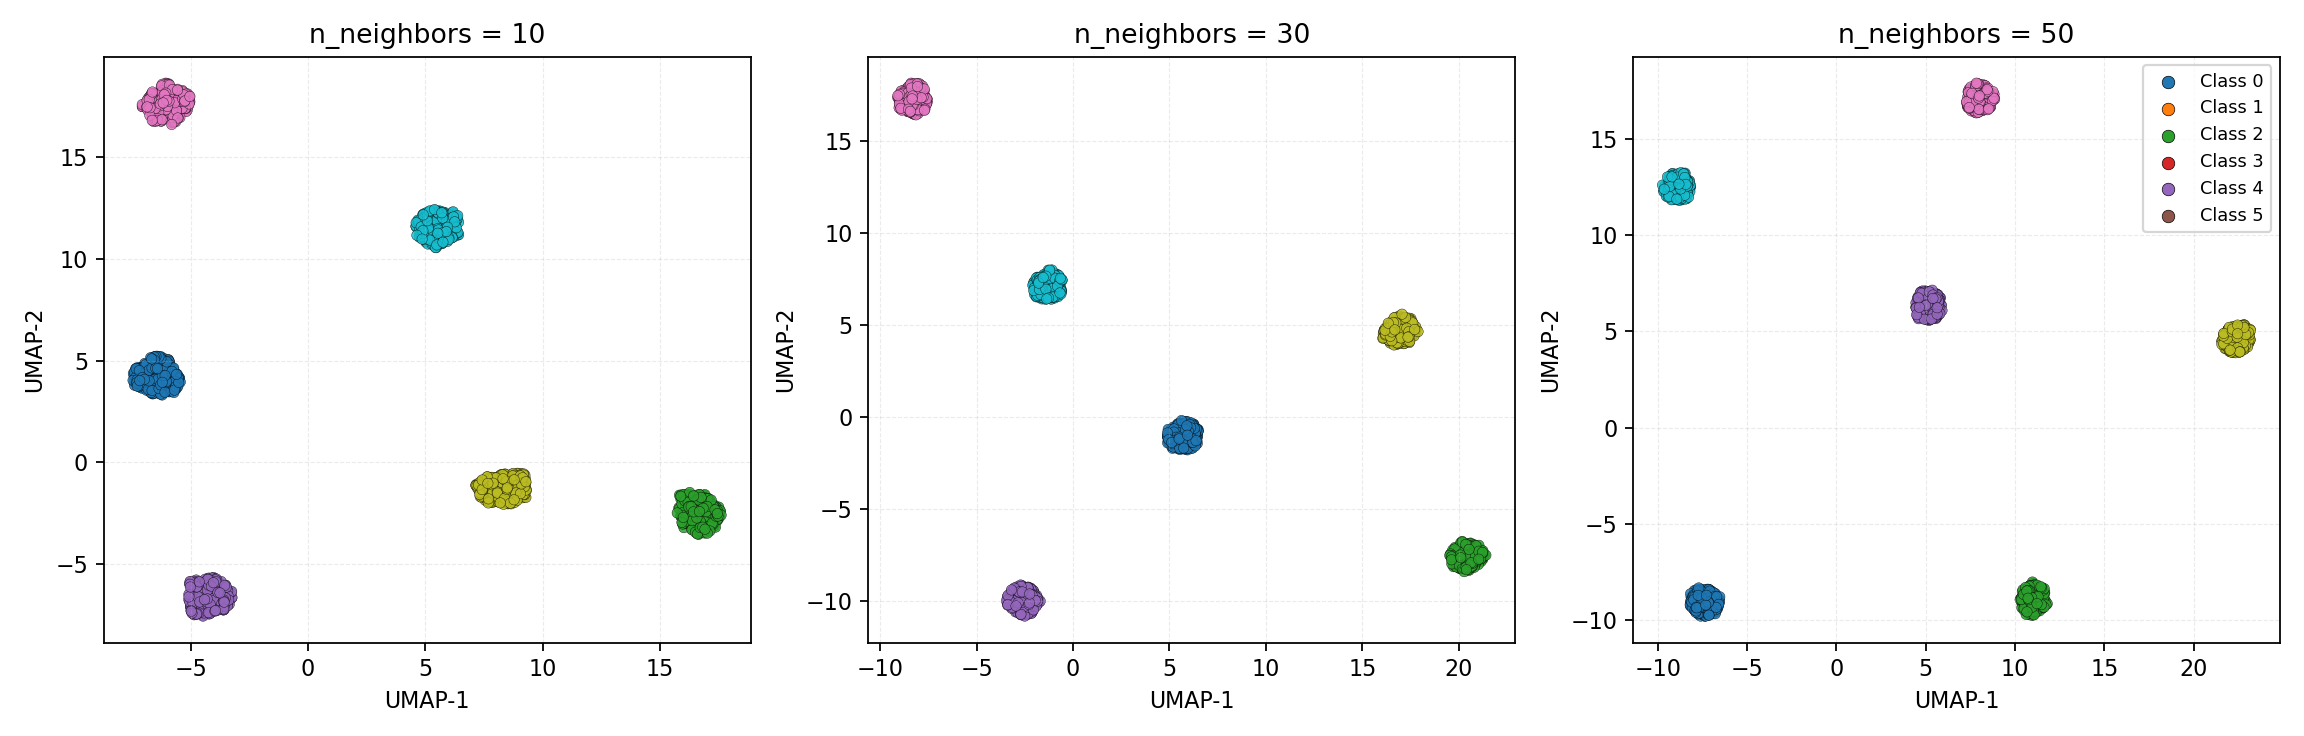
\includegraphics[width=0.82\linewidth]{umap_embeddings.png}
  \caption{UMAP embeddings for multiple neighbor counts with color-coding by class}
  \label{fig:umap_embeddings}
\end{figure}

\begin{figure}[H]
  \centering
  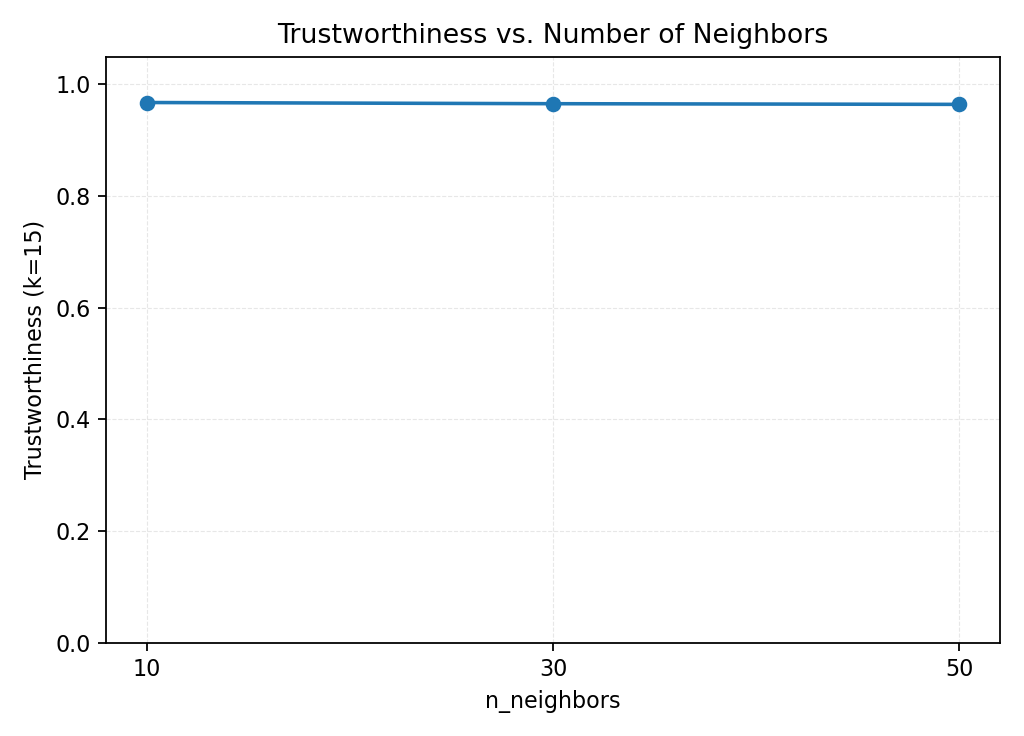
\includegraphics[width=0.8\linewidth]{umap_neighbor_curve.png}
  \caption{Trustworthiness versus number of neighbors}
  \label{fig:umap_neighbor_curve}
\end{figure}

\FloatBarrier
\section{Summary}
UMAP models neighborhood connectivity as fuzzy sets and optimizes a low-dimensional layout via cross-entropy minimization. Adjusting neighbor count, minimum distance, and metrics enables flexible trade-offs between local detail and global arrangement. The example demonstrates how to compare embeddings and monitor trustworthiness across parameter sweeps.

\end{document}